\documentclass[es,boletin]{uah}

\tema{5}
\titulo{Transmisión digital en banda base}{Baseband digital transmission}
%
\begin{document}

\titulacion{Grados TIC}
\asignatura{Teoría de la Comunicación}{Communication Theory}
\departamento{Teoría de la Señal y Comunicaciones}
\curso{2022/2023} % Do not show year

\maketitle

\seccion{Conceptos a repasar}{Key concepts}
\texto{
Antes de hacer estos ejercicios es importante repasar y tener claros los siguientes conceptos teóricos:

\begin{itemize}
\item Esquema general de un sistema de comunicaciones en banda base, incluyendo el esquema del receptor. 
\item Modulación PAM. Cálculo de la densidad espectral de potencia de una señal PAM. 
\item Códigos de línea. Tipos de códigos de línea y diferencias entre ellos.
\item Interferencia entre símbolos (ISI). Concepto de filtro ideal de Nyquist. Filtro de coseno alzado. 
\item Diagrama de ojos. Cómo se construye.
\end{itemize}
}
{
	Before doing these exercises it is important to review and understand the following concepts:	

	\begin{itemize}
	\item General scheme of a baseband communications system, including the scheme of the receiver.
	\item PAM modulation. Calculation of the power spectral density of a PAM signal.
	\item Line codes. Types of line codes and differences among them.
	\item Intersymbol Interference (ISI). Concept of Nyquist ideal filter. Raised cosine filter.
	\item Eye diagram. How it is built.
	\end{itemize}
}

%%%%%%%%%%%%%%%%%%%%%%%%%%%%%%%%%%%%%%%%%%%%%%%%%%%%%%%%
%%%%%%%%%%%%%%%%%%%%%%%%%%%%%%%%%%%%%%%%%%%%%%%%%%%%%%%%
\seccion{Problemas básicos}{Basic problems}
%%%%%%%%%%%%%%%%%%%%%%%%%%%%%%%%%%%%%%%%%%%%%%%%%%%%%%%%
%%%%%%%%%%%%%%%%%%%%%%%%%%%%%%%%%%%%%%%%%%%%%%%%%%%%%%%%
\texto{
	Este primer bloque de problemas son problemas extraídos en su mayoría de la bibliografía de la asignatura, y consisten en algunos cálculos básicos que es necesario dominar.

}
{
	This first part includes problems mostly extracted from the bibliography aimed at practicing basic calculations needed for the rest of the lesson.

}




\Problema{
	Un sistema de transmisión cuaternario en banda base transmite la siguiente señal:

\begin{displaymath}
	x(t) = \sum_{n=-\infty}^{\infty} a_n \cdot h(t-nT)
\end{displaymath}

\begin{enumerate}
	\item ¿Cuál es la base ortonormal que permite definir el espacio de señal para esta modulación?
	\item Representa la constelación.
 	\item ¿Cómo se podría calcular la probabilidad de error?
\end{enumerate}
}
{
\begin{enumerate}
	\item El propio pulso $h(t)$, normalizado si es necesario.
 	\item Constelación 4-aria unidimensional.
  \item Con la fórmula para una M-aria unidimensional. 
\end{enumerate}
}
{
	A baseband quaternary transmission system transmits the following signal:

	\begin{displaymath}
		x(t) = \sum_{n=-\infty}^{\infty} a_n \cdot h(t-nT)
	\end{displaymath}

	\begin{enumerate}
		\item Which is the orthonormal basis that can be used for this modulation?
  \item Represent the constellation
  \item How could be calculate the probability of error?
	\end{enumerate}
}
{
	\begin{enumerate}
		\item The pulse $h(t)$, normalized if necessary.
		 \item A 4-ary unidimensional constellation
	  \item With the equation for a M-ary unidimensional constellation.
	\end{enumerate}
}
%%%%%%%%%%%%%
%PROBLEMA 1-1
%%%%%%%%%%%%%
\Problema{
\cite{Carlson} Un ordenador genera palabras binarias de $16$ bits a la velocidad de $20000$ palabras por segundo. 

\begin{enumerate}
	\item Calcule el ancho de banda mínimo necesario para transmitir la salida como una señal PAM binaria.
	\item Calcule $M$ para que la salida se pueda transmitir como señal $M$-aria en un canal de $B=60 kHz$.
\end{enumerate}
}
{	
\begin{enumerate}
	\item $B_T \geq 160kHz$
	\item $M=8$
\end{enumerate}
}
{
\cite{Carlson} A computer generates $16$-bits binary words, at $20000$ words per second. 

\begin{enumerate}
	\item Calculate the bandwidth necessary for transmitting the output as a PAM binary signal.
	\item Calculate $M$ so the output can be transmitted as an $M$-ary signal in a channel with $B=60 kHz$.
\end{enumerate}
}
{
\begin{enumerate}
	\item $B_T \geq 160kHz$
	\item $M=8$
\end{enumerate}
}

%%%%%%%%%%%%%
%PROBLEMA 1-2A
%%%%%%%%%%%%%
\Problema{
Un sistema de transmisión en banda base transmite la siguiente señal:

\begin{displaymath}
	x(t) = \sum_{n=-\infty}^{\infty} a_n \cdot h(t-nT)
\end{displaymath}

donde $T$ es el intervalo de símbolo, $a_n$ es una secuencia equiprobable incorrelada cuyo valor máximo es $A$ y $h(t)$ es un pulso cuadrado normalizado en energía de duración $T_x$. 

Calcular la densidad espectral de potencia y el ancho de banda de la señal transmitida para los siguientes casos:

\begin{enumerate}
	\item Secuencia polar NRZ.
 	\item Secuencia polar RZ con $T_x = T/2$
  	\item Secuencia unipolar NRZ.
\end{enumerate}
	
}
{
\begin{enumerate}
	\item $S_x(\omega) = \frac{1}{T} \cdot \frac{1}{T} \frac{4 \sen^2\left ( \omega \frac{T}{2}\right )}{\omega^2} \cdot A^2$ \\
			$B = \frac{2\pi}{T}$
	\item $S_x(\omega) = \frac{1}{T} \cdot \frac{2}{T} \frac{4 \sen^2\left ( \omega \frac{T}{4}\right )}{\omega^2} \cdot A^2$ \\
			$B = \frac{4\pi}{T}$
	\item $S_x(\omega) = \frac{1}{T} \cdot \frac{4 \sen^2\left ( \omega \frac{T}{2}\right )}{\omega^2} \cdot \frac{A^2}{4} + \frac{A^2 \pi}{2} \delta(\omega)$ \\
			$B = \frac{2\pi}{T}$
\end{enumerate}
}
{
	A baseband transmission system transmits the following signal:

	\begin{displaymath}
		x(t) = \sum_{n=-\infty}^{\infty} a_n \cdot h(t-nT)
	\end{displaymath}
	
	where $T$ is the symbol period, $a_n$ is an equiprobable, uncorrelated sequence whose maximum value is $A$ and $h(t)$ is a normalized squared pulse with length $T_x$. 
	
	Calculate the power spectral density and the bandwidth of the transmitted signal for the following cases:
	
	\begin{enumerate}
		\item NRZ Polar sequence.
		 \item RZ Polar sequence with $T_x=T/2$.
		 \item NRZ Unipolar sequence.
	\end{enumerate}
	
}
{
	\begin{enumerate}
		\item $S_x(\omega) = \frac{1}{T} \cdot \frac{1}{T} \frac{4 \sen^2\left ( \omega \frac{T}{2}\right )}{\omega^2} \cdot A^2$ \\
				$B = \frac{2\pi}{T}$
		\item $S_x(\omega) = \frac{1}{T} \cdot \frac{2}{T} \frac{4 \sen^2\left ( \omega \frac{T}{4}\right )}{\omega^2} \cdot A^2$ \\
				$B = \frac{4\pi}{T}$
		\item $S_x(\omega) = \frac{1}{T} \cdot \frac{4 \sen^2\left ( \omega \frac{T}{2}\right )}{\omega^2} \cdot \frac{A^2}{4} + \frac{A^2 \pi}{2} \delta(\omega)$ \\
				$B = \frac{2\pi}{T}$
	\end{enumerate}
}


%%%%%%%%%%%%%
%PROBLEMA 1-2B
%%%%%%%%%%%%%
\Problema{
Un sistema de transmisión en banda base transmite la siguiente señal:

\begin{displaymath}
	x(t) = \sum_{n=-\infty}^{\infty} a_n \cdot h(t-nT)
\end{displaymath}

donde $T$ es el intervalo de símbolo, $a_n$ es una secuencia equiprobable incorrelada cuyo valor máximo es $A$ y $h(t)$ es un pulso en coseno alzado con \emph{roll-off factor} -exceso de ancho de banda- $\alpha$. 

Calcular la densidad espectral de potencia y el ancho de banda de la señal transmitida suponiendo que se utiliza una codificación polar.
	
}
{
	$S_x(\omega) = \frac{1}{T} \cdot |H(\omega)|^2 \cdot A^2$, siendo $H(\omega)$ la respuesta en frecuencia del filtro en coseno alzado. \\
			$B = \frac{1+\alpha}{2T}$
}
{
	A baseband transmission system transmits the following signal:

	\begin{displaymath}
		x(t) = \sum_{n=-\infty}^{\infty} a_n \cdot h(t-nT)
	\end{displaymath}
	
	where $T$ is the symbol period, $a_n$ is an equiprobable, uncorrelated sequence whose maximum value is $A$ and $h(t)$ is a raised cosine pulse with roll-off factor $\alpha$. 
	
	Calculate the power spectral density and the bandwidth of the transmitted signal assuming polar coding.
	
}
{
	$S_x(\omega) = \frac{1}{T} \cdot |H(\omega)|^2 \cdot A^2$, with $H(\omega)$ being the frequency response of the raised cosine filter. \\
				$B = \frac{1+\alpha}{2T}$

}



%%%%%%%%%%%%%
% PROBLEMA 1-3
%%%%%%%%%%%%%
\Problema
{
Considere una secuencia binaria $b_n$ a partir de la cual formamos los símbolos $a_n= b_n - b_{n-1}$, los $b_n$ son variables aleatorias binarias equiprobables e incorreladas, que toman los valores $1$ y $0$. 

Calcule el ancho de banda y la densidad espectral de potencia de la señal transmitida para el caso en que el filtro transmisor tenga una respuesta al impulso:

\begin{displaymath}
	h_T(t) = \left \{ \begin{array}{ll}
		\frac{1}{\sqrt{T}} & 0 \leq t < T \\
		0 & c.c. \\
	\end{array} \right.
\end{displaymath}
}
{
\begin{enumerate}
\item $S_x(\omega) = \frac{4}{T^2 \omega^2} sen^4 \left ( \frac{\omega T}{2} \right )$
\item $B = \frac{2\pi}{T}$
\end{enumerate}
}
{
Consider a binary sequence $b_n$, from which we form the symbols $a_n= b_n - b_{n-1}$, $b_n$ are uncorrelated and equiprobable random variables, taking values $1$ and $0$. 

Calculate the power spectral density of the transmitted signal, in the case that the transmitter filter is:

\begin{displaymath}
	h_T(t) = \left \{ \begin{array}{ll}
		\frac{1}{\sqrt{T}} & 0 \leq t < T \\
		0 & c.c. \\
	\end{array} \right.
\end{displaymath}
}
{
$S_x(\omega) = \frac{4}{T^2 \omega^2} sen^4 \left ( \frac{\omega T}{2} \right )$
}


%%%%%%%%%%%%%
% PROBLEMA 1-4
%%%%%%%%%%%%%
\Problema{
\cite{Carlson} Calcule la $\left ( \frac{S}{N} \right )_R$ para que un sistema binario unipolar con ruido blanco gaussiano aditivo tenga $P_e= 0.001$. 

¿Cuál será la probabilidad de error de un sistema polar con la misma $\left ( \frac{S}{N} \right )_R$.
}
{
\begin{enumerate}
	\item $\rho = \frac{E_s}{N_0/2} = 19,22$ \\
		$P_e = Q(4,38) < 8.54 \cdot 10^{-6}$
\end{enumerate}
}
{
\cite{Carlson} Calculate the $\left ( \frac{S}{N} \right )_R$ such that a binary unipolar system with white Gaussian noise has a $P_e= 0.001$. 

What is the error probability of a polar system with the same $\left ( \frac{S}{N} \right )_R$?
}
{
\begin{enumerate}
	\item $\rho = \frac{E_s}{N_0/2} = 19,22$ \\
		$P_e = Q(4,38) < 8.54 \cdot 10^{-6}$
\end{enumerate}
}

%%%%%%%%%%%%%%%%
% PROBLEMA 1-5
%%%%%%%%%%%%%%%%%
\Problema{
\cite{Haykin} Considere la señal $h_{TC}(t)$ de la figura:

{\begin{figure*}[h!]\centering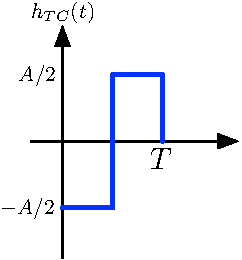
\includegraphics[width=4cm]{./Figuras/Problema5_4}\end{figure*}}

\begin{enumerate}
	\item Determine la respuesta al impulso del filtro adaptado a esta señal y represéntela en función del tiempo.
	\item Dibuje la forma de onda de la respuesta al impulso global $h(t)$.
\end{enumerate}
}
{
\begin{enumerate}
	\item $h_R(t) = h_{TC}(T-t)$
	\item \
	{\begin{figure*}[h!]\centering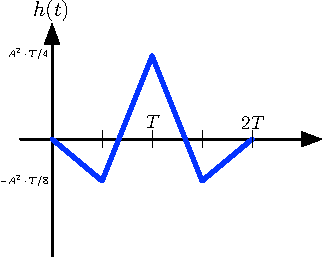
\includegraphics[width=4cm]{./Figuras/Problema5_4_sol}\end{figure*}}
\end{enumerate}
}
{
\cite{Haykin} Consider the signal $h_{TC}(t)$ in the figure:

{\begin{figure*}[h!]\centering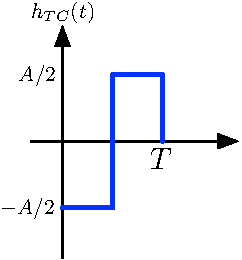
\includegraphics[width=4cm]{./Figuras/Problema5_4}\end{figure*}}

\begin{enumerate}
	\item Determine the impulse response of the matched filter to that signal, and draw it in function of the time.
	\item Draw the waveform of the global impulse response $h(t)$.

\end{enumerate}
}
{
\begin{enumerate}
	\item $h_R(t) = h_{TC}(T-t)$
	\item \
	{\begin{figure*}[h!]\centering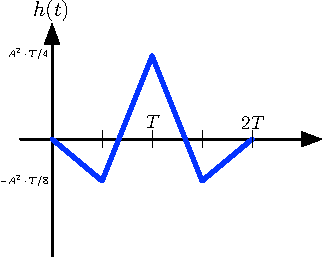
\includegraphics[width=4cm]{./Figuras/Problema5_4_sol}\end{figure*}}
\end{enumerate}
}

%%%%%%%%%%%%%%%%
% PROBLEMA 1-6
%%%%%%%%%%%%%%%%%
\Problema{
\cite{Carlson}  Se recibe una señal PAM $r(t)=\sum_{n=-\infty}^{\infty} b_n h(t-nT)$.

 Dibuje dicha señal $r(t)$ y construya su diagrama de ojos, sin distorsión, para la siguiente secuencia de datos en formato unipolar: $1011100010$. 
 
 \begin{displaymath}
 	h(t) = cos^2 \left ( \frac{2\pi}{4T_b} t \right ) \prod \left ( \frac{t}{2T_b} \right )
 \end{displaymath}
}
{
\begin{center}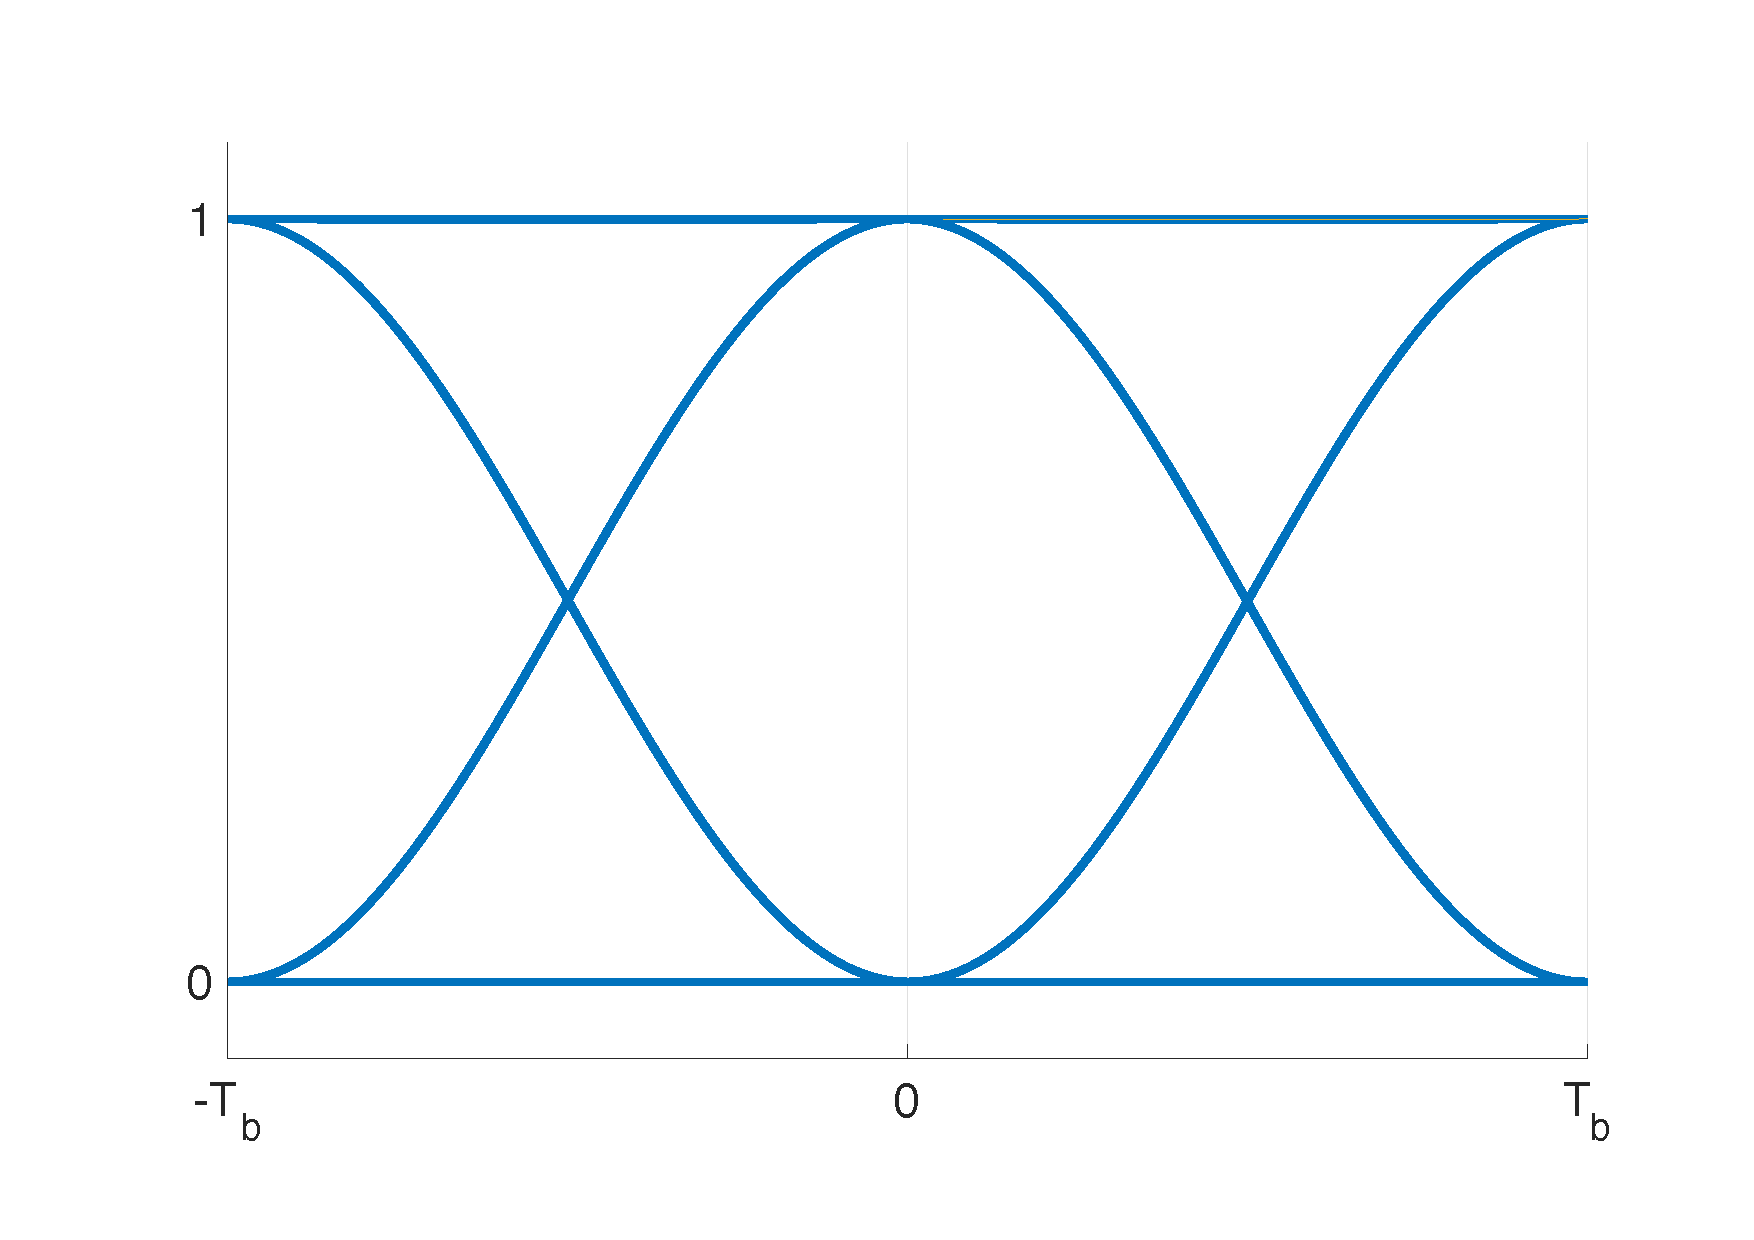
\includegraphics[width=8cm]{./Figuras/Problema5_5_sol}\end{center}
}
{
\cite{Carlson} The following PAM signal is received:  $r(t)=\sum_{n=-\infty}^{\infty} b_n h(t-nT)$.

 Draw and determine its eye pattern, without distortion, considering the following unipolar data sequence: $1011100010$. 
 
 \begin{displaymath}
 	h(t) = cos^2 \left ( \frac{2\pi}{4T_b} t \right ) \prod \left ( \frac{t}{2T_b} \right )
 \end{displaymath}
}
{
\begin{center}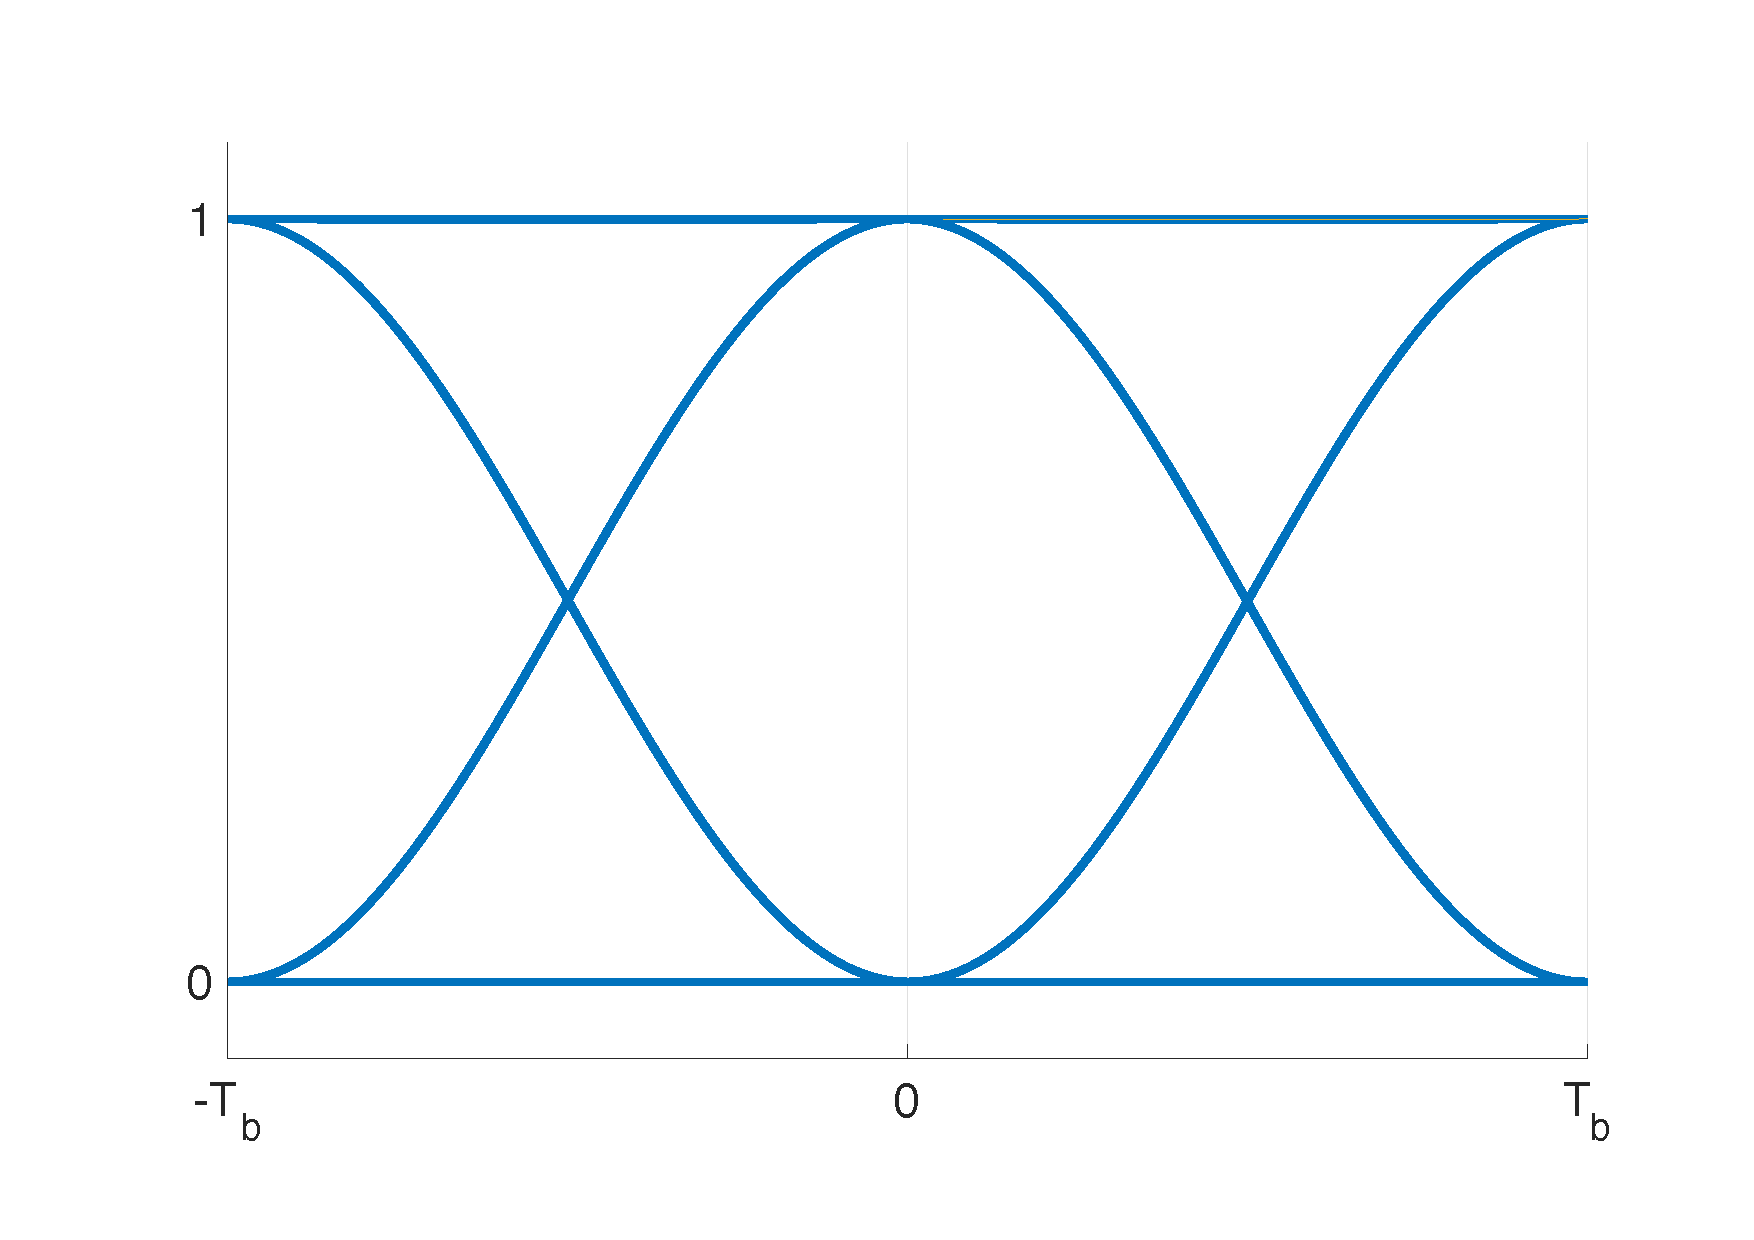
\includegraphics[width=8cm]{./Figuras/Problema5_5_sol}\end{center}
}

%%%%%%%%%%%%%%%%
% PROBLEMA 1-7
%%%%%%%%%%%%%%%%%
\Problema{
Un ordenador genera impulsos con una tasa de $R_b = 1 Mbps$, para su transmisión por un canal ruidoso con densidad espectral de potencia $N_0/2 = 2\cdot 10^{-20} W/Hz$. Se especifica que la tasa de error no debe superar el valor de $1$ bit por hora. Se pide:

\begin{enumerate}
	\item Determinar la potencia de ruido del canal y la probabilidad de error de bit en el sistema.
	\item Supóngase que en el transmisor se incluye ahora una característica de transferencia con espectro en coseno alzado, con un exceso de ancho de banda del $75\%$, y que el sistema sea PAM cuaternario. Calcular el nuevo ancho de banda necesario para la transmisión.
\end{enumerate}
}
{
\begin{enumerate}
	\item $P_N = 2 \cdot 10^{-14} W$, $P_b = 2.7 \cdot 10^{-10}$
	\item $B=437.5 kHz$
\end{enumerate}
}
{
A computer generates pulses with $R_b = 1 Mbps$, for their transmission through a noisy channel, with power spectral density $N_0/2 = 2\cdot 10^{-20} W/Hz$. The error rate cannot be over 1 bit per hour.

\begin{enumerate}
	\item Determine the noise power of the channel and the error probability of the system.
	\item Suppose that the transmitter includes now a transfer characteristic using a raised cosine spectrum, with an excess of bandwidth of $75\%$, and the systems is PAM quaternary. Calculate the new bandwidth necessary for the transmission.
\end{enumerate}
}
{

\begin{enumerate}
	\item $P_N = 2 \cdot 10^{-14} W$, $P_b = 2.7 \cdot 10^{-10}$
	\item $B=437.5 kHz$
\end{enumerate}
}



%%%%%%%%%%%%%%%%%%%%%%%%%%%%%%%%%%%%%%%%%%%%%%%%%%%%%%%%
%%%%%%%%%%%%%%%%%%%%%%%%%%%%%%%%%%%%%%%%%%%%%%%%%%%%%%%%
\newpage
\seccion{Problemas adicionales}{Aditional problems}
%%%%%%%%%%%%%%%%%%%%%%%%%%%%%%%%%%%%%%%%%%%%%%%%%%%%%%%%
%%%%%%%%%%%%%%%%%%%%%%%%%%%%%%%%%%%%%%%%%%%%%%%%%%%%%%%%
\texto{
	Estos problemas son algo más elaborados que los anteriores, en muchos casos extraídos de exámenes antiguos.

}
{
	These problems are slightly more ellaborated than the previous ones, in many cases extracted from old exams.

}
%%%%%%%%%%%%%
%PROBLEMA 2-1
%%%%%%%%%%%%%
\Problema{

Un sistema de comunicación digital tiene transmite la señal:

\begin{displaymath}
s(t) = \sum_{n=-\infty}^{\infty} b_n \cdot h_T(t-nT)
\end{displaymath}

donde $b_n$ representa una secuencia de variables aleatorias discretas, independientes e idénticamente distribuidas (iid) que toman valores $\pm 1$ con la misma probabilidad. La forma de onda del impulso transmitido es $h(t) = \frac{1}{\sqrt{T}} \cdot \prod \left ( \frac{t-T/2}{T} \right )$, la respuesta al impulso del canal es $h_c(t)=\delta (t)$ y el filtro receptor $h_R(t)$ está adaptado a $h_T(t)$. Se pide:

\begin{enumerate}
	\item Determinar la forma de onda de la respuesta al impulso global $h(t)$.
	\item Dibujar el diagrama de ojos de la señal de salida del filtro receptor antes de ser muestrada.
	\item Repetir el apartado a) para un canal con respuesta al impulso $h_c(t)=\delta (t) - 0.5 \cdot \delta (t-T)$.
	\item Calcular los valores de las muestras de la señal tomadas a la salida del filtro receptor, así como el valor de la interferencia entre símbolos (ISI) en cada una de ellas suponiendo que se ha transmitido la secuencia $1101$.
\end{enumerate}

\textsc{Nota:} $\prod(t) = \left \{ \begin{array}{ll} 1 & -0.5\leq t <0.5 \\ 0 & c.c. \\
 \end{array} \right.$
 \ \\

}
{

\begin{tabular}[h]{cc}
	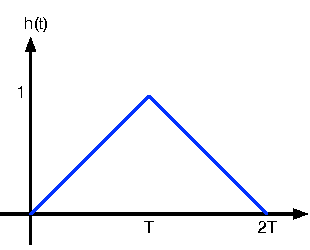
\includegraphics[height=2.5cm]{./Figuras/Problema5_9a} &
	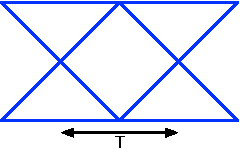
\includegraphics[height=1.75cm]{./Figuras/Problema5_9b} \\
	Apartado (a) & Apartado (b) \\
	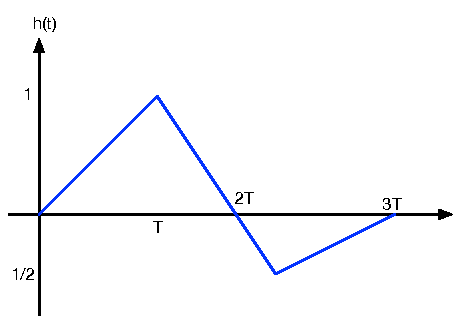
\includegraphics[height=2.5cm]{./Figuras/Problema5_9c} &
	\\
	Apartado (c) & \\
\end{tabular}

}
{

A communication system transmits the following signal:

\begin{displaymath}
s(t) = \sum_{n=-\infty}^{\infty} b_n \cdot h_T(t-nT)
\end{displaymath}

where $b_n$ represents a sequence of discrete random variables, independent and identically distributed, which take the values $\pm 1$ with the same probability. The transmitted pulse is $h(t) = \frac{1}{\sqrt{T}} \cdot \prod \left ( \frac{t-T/2}{T} \right )$, the channel impulse response is $h_c(t)=\delta (t)$ and the receiver filter $h_R(t)$ is matched to $h_T(t)$. 

\begin{enumerate}
	\item Determine the wave form of the global impulse response $h(t)$.
	\item Draw the eye diagram of the receiver filter output, before sampling.
	\item Repeat a) for a channel with impulse response $h_c(t)=\delta (t) - 0.5 \cdot \delta (t-T)$.
	\item Calculate the values of the samples at the receiver filter output, and the value of the inter-symbol interference in each of them.
\end{enumerate}

\textsc{Note:} $\prod(t) = \left \{ \begin{array}{ll} 1 & -0.5\leq t <0.5 \\ 0 & c.c. \\
 \end{array} \right.$
 \ \\

}
{

\begin{tabular}[h]{cc}
	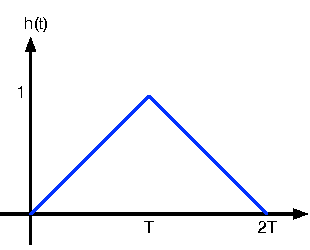
\includegraphics[height=2.5cm]{./Figuras/Problema5_9a} &
	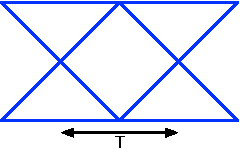
\includegraphics[height=1.75cm]{./Figuras/Problema5_9b} \\
	Apartado (a) & Apartado (b) \\
	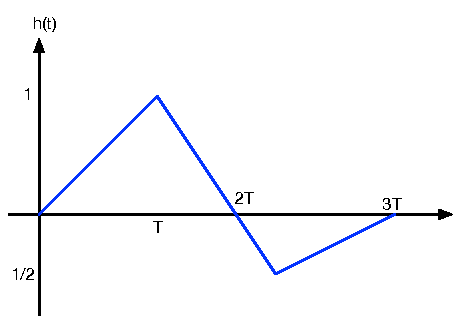
\includegraphics[height=2.5cm]{./Figuras/Problema5_9c} &
	\\
	Apartado (c) & \\
\end{tabular}

}




\Problema{
	[Examen2012] Considere un sistema de comunicación digital binario que transmite un código polar NRZ con la forma de impulso $h_{TC}(t)$ de la figura. 

\begin{center}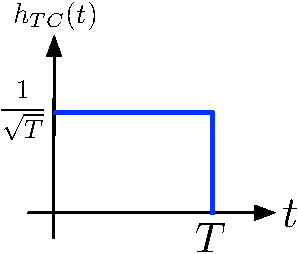
\includegraphics[width=4cm]{Figuras/Problema5_10}\end{center}

\begin{enumerate}
	\item Determine la respuesta al impulso del filtro adaptado y represente en función del tiempo la salida del mismo cuando se recibe un \bits{1} y cuando se recibe un \bits{0}.
 \item Calcule la probabilidad media de error de detección en un canal de ruido blanco gaussiano aditivo, cuya densidad espectral de potencia de ruido sea $N_0/2$ W/Hz.
\end{enumerate}

{\bf Datos:} Energía media por bit $E_b = 4 \,\textrm{pJ}$, $N_0 = 3.6\cdot 10^{-13} \,\textrm{W/Hz}$.
}
{
	\begin{enumerate}
		\item \ \\
		\begin{center}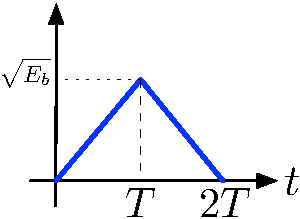
\includegraphics[width=4cm]{Figuras/Problema5_10b}\end{center}
  		\item $P_e = 1.3 \cdot 10^{-6}$ 
	\end{enumerate}
}
{
	[Exam2012] Consider a binary digital communication system that transmits an NRZ polar code with the pulse shape $h_{TC}(t)$ in the figure.

	\begin{center}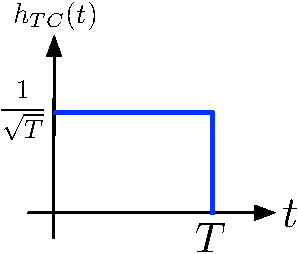
\includegraphics[width=4cm]{Figuras/Problema5_10}\end{center}

\begin{enumerate}
	\item Determine the impulse response of the matched filter and plot the output of the matched filter as a function of time when a \bits{1} is received and when a \bits{0} is received.
	\item Compute the mean probability of detection error in an additive white Gaussian noise channel, whose noise power spectral density is $N_0/2$ W/Hz.
\end{enumerate}

{\bf Data:} Mean bit energy $E_b = 4 \,\textrm{pJ}$, $N_0 = 3.6\cdot 10^{-13} \,\textrm{W/Hz}$.
}
{
	\begin{enumerate}
		\item \ \\
		\begin{center}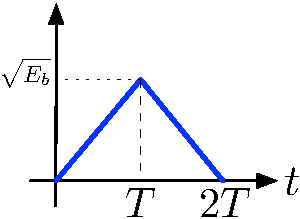
\includegraphics[width=4cm]{Figuras/Problema5_10b}\end{center}
  		\item $P_e = 1.3 \cdot 10^{-6}$ 
	\end{enumerate}
}


\Problema{
	[Examen2012] Un dispositivo electrónico genera $30000$ palabras binarias por segundo, que son transmitidas como una señal PAM-binaria unipolar NRZ con $10\,\textrm{mV}$ de amplitud de pulso a la entrada del canal, cuyo ancho de banda es $120\,\textrm{kHz}$, que atenúa la señal $10\,\textrm{dB}$ e introduce ruido blanco gaussiano de densidad espectral de potencia $N_0/2 = 10^{-10}\,\textrm{W/Hz}$.

	\begin{enumerate}
\item Número de bits máximo, $n$, que tiene cada palabra binaria. Se supone que todas las palabras generadas tienen igual número de bits.
\item Energía media de símbolo a la salida del canal, considerando que los símbolos son equiprobables. 
	\end{enumerate}

	Si por razones económicas se reduce el ancho de banda del canal a $60 \,\textrm{kHz}$.

	\begin{enumerate}
		\setcounter{enumi}{2}
\item Determinar el valor de $M$ para que la salida se pueda transmitir como señal M-aria.
	\end{enumerate}

	Si por razones de diseño se incluye en el transmisor una característica de transferencia con espectro en coseno alzado, con un exceso de ancho de banda del $95\%$ y la salida se transmite como señal 8-aria.
	
	\begin{enumerate}
		\setcounter{enumi}{3}
\item Determinar el nuevo ancho de banda necesario para la transmisión
	\end{enumerate}
	}
	{
	\begin{enumerate}
		\item $n=8$
   		\item $E_s = 2.083\cdot 10^{-11}\,\textrm{J}$
     	\item  $M=4$
      \item $B_T = 78 \,\textrm{kHz}$
	\end{enumerate}
	}
	{
		[Exam2012] An electronic device generates $30000$ binary words per second, which are transmitted as a unipolar NRZ PAM-binary signal with $10\,\textrm{mV}$ pulse level at the input of the channel, whose bandwidth is $120\, \textrm{kHz}$, which attenuates the signal by $10\,\textrm{dB}$ and introduces Gaussian white noise of power spectral density $N_0/2 = 10^{-10}\,\textrm{W/Hz} $.

	\begin{enumerate}
		\item Maximum number of bits, $n$, that each binary word has. All generated words are assumed to have the same number of bits.
		\item Average symbol energy at the channel output, considering that the symbols are equiprobable.
	\end{enumerate}

	If for economic reasons the channel bandwidth is reduced to $60 \,\textrm{kHz}$.

	\begin{enumerate}
		\setcounter{enumi}{2}
		\item Determine the value of $M$ so that the output can be transmitted as an M-ary signal.
	\end{enumerate}

	If for design reasons a transfer characteristic with raised cosine spectrum is included in the transmitter, with an excess of bandwidth of $95\%$ and the output is transmitted as an 8-ary signal.
	
	\begin{enumerate}
		\setcounter{enumi}{3}
\item Determine the new bandwidth needed for transmission
	\end{enumerate}
	}{
		\begin{enumerate}
			\item $n=8$
			   \item $E_s = 2.083\cdot 10^{-11}\,\textrm{J}$
			 \item  $M=4$
		  \item $B_T = 78 \,\textrm{kHz}$
		\end{enumerate}
	}



\begin{thebibliography}{100}
\bibitem[Carlson2010]{Carlson} A. Bruce Carlson and Paul B. Crilly. Communication Systems: An Introduction to Signals and Noise in Electrical Communication, 5th Ed. McGraw-Hill, 2010.
\bibitem[Haykin2001]{Haykin}  Simon Haykin. Communication Systems, 4th Ed. John Wiley and Sons, 2001.
\end{thebibliography}






\end{document}



	
